\section{Introduction}
\label{lo:sec:introduction}

Numerical C programs typically spend most of their time in loops.  For this
reason, \gls{hls} tools adopt state-of-the-art \emph{polyhedral compilation}
techniques~\cite{canis14} to synthesize loops to run as fast as possible.  This
is achieved by pipelining them to maximally exploit parallelism across loop
iterations.  Certain program transformations, such as conventional program
equivalences (\eg~partial loop unrolling and array access pattern changes) are
highly ubiquitous in their compilation process.

However, their ability to perform pipelining, even with any combinations of
these equivalences, is fundamentally constrained by data-dependences that
are carried across iterations, \ie~\emph{inter-iteration dependences}.  To
relax these constraints, we must use equivalence rules in real arithmetic
(\eg~associativity and distributivity), in tandem with the conventional rules
above to enable much more efficiently pipelined \gls{rtl} designs.  A simple
example of this is the summation of all elements in an array:
\begin{lstlisting}
  float sum = 0;
  for (int i = 0; i < N; i++)
    sum += a[i];
\end{lstlisting}
This code can be partially unrolled and the sequence of additions can be
rewritten using tree adders to reduce its latency, but we will see later in
Section~\ref{lo:sec:results} that more efficient implementations are possible.

In contrast to the expression balancing optimization pass in \gls{vhls}, the
new \soap~in this chapter \emph{automatically} produces results that are
significantly better than \emph{manually} tuning partial unrolling factors
and expression balancing \verb|#pragma|s in \gls{vhls}, because it is fully
aware of how data-dependences are carried across iterations, and uses this
to steer the optimization process. \soap~is also fully aware of the impact
these transformations could have on round-off errors, and minimizes them in
the optimization process, as we treat numerical accuracy as one of the three
simultaneous objectives.  Furthermore, \gls{vhls} only generates one result
which does not necessarily improve over the original code.

The technical work presented in Chapters~\ref{chp:stropt} and~\ref{chp:progopt}
lays the necessary foundation for the new methods proposed in this chapter.
Firstly, we exploit the \soap~framework's ability to analyze the numerical
accuracy of a given program.  Secondly, the framework provides the basis for
resource analysis, as common subexpression sharing can be detected by the
method detailed in Section~\ref{po:sec:resource} of Chapter~\ref{chp:stropt}.
Thirdly, we can make use of \glspl{mir} to explore program rewrites.  Finally,
the efficient algorithms for equivalent program discovery in \soap~can be
readily used.

In previous chapters, we only analyze structural reuse in the form of common
subexpressions.  HLS tools further allows certain arithmetic operations to be
shared temporally.  In this chapter, we therefore additionally analyze resource
utilization by considering the implications of sharing the same resources in
different clock cycles.  For this purpose, we use a variant of the first few
steps shared by modulo \gls{sdc} scheduling~\cite{canis14} and \acrfull{ims}
algorithm~\cite{rau94}, which efficiently analyze the run time and resource
utilization of a given program, by computing fundamental lower bounds of these
metrics.

\soap~is evaluated on a suite of 11 programs from the Livermore
Loops~\cite{livermore} and PolyBench~\cite{polybench} benchmark suites.  Our
tool obtained a wide selection of Pareto-optimized programs.  Programs with
the best latency obtained speedups of up to $12\times$ ($7\times$ on average
across the suite), and increases in accuracy of up to $7\times$ ($2.7\times$
on average), while using up to $4\times$ ($2.5\times$ on average) more
\glspl{lut}.  We were unable to decrease the resource utilization in any of the
benchmarks, as they have no redundant computations.

The contributions of this chapter include:
\begin{itemize}

    \item An extended suite of program equivalence rules, which introduces
    access reduction rules that removes extraneous array accesses.  This
    chapter provides evidence that standard program equivalence that do not
    affect program behavior, \eg~partial loop unrolling and access reduction
    rules, can give rise to the freedom for non-standard transformation rules,
    \eg~arithmetic rules, to significantly impact latency, resource usage and
    accuracy in a loop (Section~\ref{lo:sub:transformation_rules}).

    \item A new scheduling analysis that estimates the
    latency and resource usage of a given optimized candidate
    (Section~\ref{lo:sec:performance_analysis}).  The resource usage analysis
    not only identifies common subexpressions, but also opportunities to share
    arithmetic operations temporally.

    \item A significantly faster efficient discovery of equivalent
    programs through a faster accuracy analysis that analyze a fraction
    of loop nest executions, speed up analysis of loop nests without
    inter-iteration dependences (Section~\ref{lo:sub:accuracy}), graph
    partitioning, and intelligent pruning of optimization candidates
    (Section~\ref{lo:sub:algorithm}).

    \item Incorporating the above-mentioned techniques, \soap{} is now
    capable of \emph{automatically} and \emph{safely} producing optimized
    programs (and subsequent \gls{rtl} implementations with \gls{vhls}) on
    the three-dimensional Pareto frontier of options that trade off run time,
    accuracy, and area.  Its improvements in latency are notably better than
    the only ones produced by \gls{vhls}'s \emph{unsafe} optimizations.
    \soap~is further evaluated on a suite of Livermore Loops and PolyBench
    benchmarks (Section~\ref{lo:sec:results}).

\end{itemize}

This chapter, which is a natural extension to previous chapters, is
organized as follows.  Section~\ref{lo:sec:motivation} details how a
simple numerical program can be optimized to run efficiently as our
motivating example.  Our automatic optimization process consists of
three major steps.  It starts by the process of \acrlong{ma}, which
takes as an input the original numerical program written in C, and
translates it into a \gls{mir}.  Section~\ref{lo:sec:intermediate}
explains how this process is extended to multi-dimensional arrays.  We
then discover equivalent \glspl{mir} using our efficient equivalent
program discovery procedure, which produces a Pareto frontier of optimized
\glspl{mir}.  Section~\ref{lo:sec:structural_optimization} discusses the
improvements made to this procedure to further increase its performance.
This process in turn makes use of the two new performance analyses in
Section~\ref{lo:sec:performance_analysis}, which respectively estimate the
latency and resource utilization.  This section further explains how round-off
errors can be bound in a given program written with arrays.  The optimized C
programs can then be generated from the \glspl{mir}, using the code generation
routines from Chapter~\ref{chp:progopt}, to be synthesized in \gls{vhls} to
obtain \gls{rtl} implementations.  In Section~\ref{lo:sec:results} we evaluate
the results of optimizing a suite of benchmark examples extracted from
PolyBench~\cite{polybench} and Livermore Loops~\cite{livermore}.

Figure~\ref{lo:fig:overview} illustrates the high-level overview of the
internal tool flow of the final iteration of \soap.
\begin{figure}[ht]
    \centering
    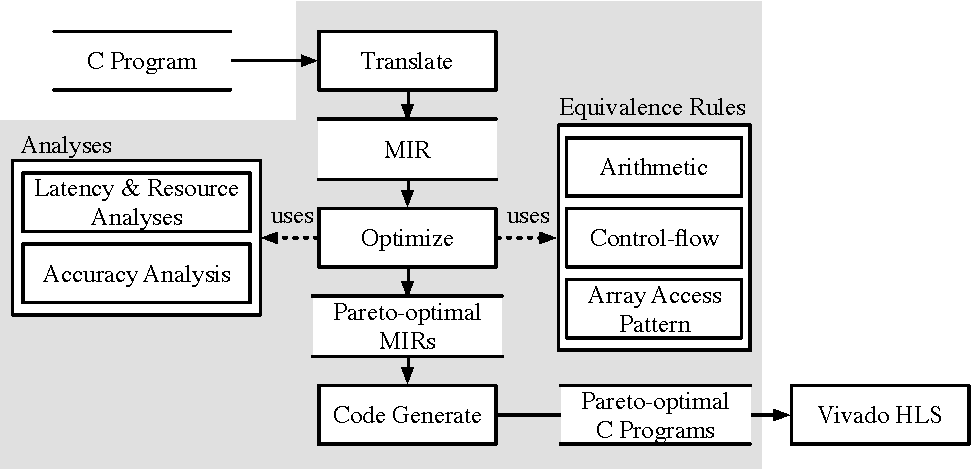
\includegraphics[scale=0.8]{overview}
    \caption{%
        An overview of our automatic program optimization process. The shaded
        region shows our internal tool flow.
    }\label{lo:fig:overview}
\end{figure}
